\chapter{Introduction to Diffeomorphic Image Registration}\label{ch:introduction}


\begin{flushright}
		\emph{The series is divergent, therefore we may be able \\ to do something with it.}\\
			- Oliver Heaviside
\end{flushright}

\vspace{0.6cm}


\section{Toward an ill-posed Problem}

The process of determining correspondences between two or more images acquired from patients scans is a challenging task that has seen the application of a growing number of mathematical theories contributing to its solution.\\
The challenge and the concomitant difficulties in approaching the problem is a consequence of the fact that dealing with image registration problem means dealing with an ill-posed problem. Transformations between anatomies are not unique, and the impossibility to recover spatial or temporal evolution of an anatomical transformation from temporally isolated images, makes any validation a difficult, if not an impossible task. 
In addition each situation inevitably brings some prior knowledge within the initial data, that may imply some modifications in the problems' setting and may imply some additional constraints. This, of course, impact dramatically the range of possible results. \\

It is often the practical situation that provides the hint in choosing the optimal constraints, but it almost never provides enough information to reduce the large amount of options involved. A wide range of variants in methodologies and approaches to solve the registration problem has been thus proposed in the last decades: a quick glance to Google scholar reveals about $1200000$ papers in \emph{medical image registration} (55\% of the whole \emph{image registration} resources). 

\subsection{Examples of applications}
One of the main application of image registration is in the domain of brain imaging: there this tool can be used to examine differences between subjects and distinguish their biological features (cross-sectional studies) or to compare different acquisition of the same subject, before and after a surgery or after a fixed period of time (longitudinal studies). \\

In both cases an accurate comparison between images and the parameters of the transformation involved may result in a quantification of anatomical variability and in a better understanding of the patients' features. 
%
For example, brain atrophy is considered a biomarker to diagnose the Alzheimer disease and to analyze its evolution; most of the algorithms and techniques involved in the atrophy measurement requires longitudinal or cross-sectional scans to be aligned, and so are directly affected by the solution of the registration algorithm (See \cite{fox1997brain}, \cite{gauthier2012prevention}, \cite{prados2015measuring} for studies on brain atrophy involving registration). \\

Also when dealing with motion correction, if a sequence of images is affected by the motion of cardiac pulses or respiratory cycles, registration algorithms are often used for the realignment. 
They are also involved, for example, in lungs radiotherapy. In this case, a the correspondence between the lungs' deformation obtained from the registration algorithms and the respiratory signal defines a model to direct the X-ray or electrons beam on the cancerous tissue. Thanks to the correspondence, the beam follow the cancerous tissue during the respiration, minimizing damages on the sane tissue \cite{mcclelland}, \cite{mcclelland2011inter}.\\

Another application of image registration is the composition of several images aided to obtain a bigger picture - this procedure is sometime called \emph{mosaicing}. In this case a registration algorithm aligns images using information obtained form the overlapping regions (See \cite{vercauteren2006robust}, \cite{szeliski1994image} as examples of image registration applied to mosaicing processes).

\subsection{Diffeomorphisms in medical imaging: State of the Art}

In the attempt to classify image registration algorithms, one of the most relevant feature that distinguish them is the choice of the family to whom the transformation belongs and its parametrization. Since anatomies are in a continuous process of modification over time, in general without any variation in the topological features, the use of diffeomorphisms (as invertible topology-preserving functions) appears to be one of the most natural choice to model organs' transformations.\\

In the development of diffeomorphic image registration, we can broadly identify some steps that led to the concept of log-composition presented in this research:
\begin{enumerate}
	\item[1981-1996 $\triangleright$] The use of diffeomorphisms in medical image registration began from the research of a solution to a class partial differential equations: deformations are modeled as the consequent effect of two balancing forces applied to an elastic body \cite{Broit:1981} or to conserve the energy momentum \cite{christensen1996deformable}. In this early stage, diffeomorphisms are the domain of the solution of a differential equation, and are not considered with their Lie group structure.
	%
	\item[1998-2004 $\triangleright$] Based on the concept of attraction, the demons algorithm \cite{thirion1998image}, \cite{pennec1999understanding} propose the computation of the transformation between images in an iterative framework, where the update of the transformation at each step is parametrized with a vector field that is optimized at each step. This vector field is defined as the set of vectors (demons) that moves each voxel of the moving image into a new position, corresponding to the fixed of the other. \\
	Here diffeomorphisms are not directly involved and the vectors at each voxel are considered as independent elements. 
	In the same year of \cite{thirion1998image}, the set of diffeomorphism was taken into account in image matching and computational anatomy, not only as the set of solutions of some family of differential equations, but with its tangent space \cite{Dupuis:98:variationalproblems,  trouve1998diffeomorphisms, grenander1998computational}.
	%
	\item[2005-2006 $\triangleright$] The almost concomitant publication of the Large Deformation Diffeomorphic Metric Mapping (LDDMM) in \cite{beg2005computing} with some investigations about the tangent space to the Lie group of diffeomorphisms as a space where to perform statistics - the so called log-Euclidean framework \cite{arsigny2006statistics, Arsigny:MRM:06} 
	bring to the attention the use of the tangent space to diffeomorphisms and to consider them as a Lie group provided by a Lie algebra.\\
	The LDDMM revealed all the opportunities provided by differential geometry in considering tangent vectors to the space of transformation in a framework for the computation of image registration. In this setting, the tangent vector field comes from the solution of the ODE that models the transformations and it consists of the set of the non-stationary vector field (also time varying vector field or TVVF). After the log-Euclidean framework \cite{arsigny2006statistics}, aimed at the computation of statistics of diffeomorphisms, the set of tangent vector field is restricted to the time-independent vector field (also stationary velocity field or SFV).
	%
	\item[2007-2013 $\triangleright$] The restriction to SVF was subsequently considered in some further improvements of LDDMM  as DARTEL and Stationary LDDMM \cite{Ashburner:07}, \cite{hernandez2007registration}. 
	Log-Euclidean framework brought new life also to the demons algorithm, that  become, in 2007, the diffeomorphic demons \cite{vercauteren2007non}.
	Subsequent approaches involving the symmetrization of the energy function and the use of a different norm (local correlation coefficient instead of $L^{2}$) are proposed in symmetric log-demons \cite{vercauteren08} and LCC-demons \cite{lorenzi2013lcc} respectively.
	
\end{enumerate}


% % % % % % % % % % % % % % % % % % % % % % % % % % % % % % % % % % % % % %
% %  SUBSECTION
% % % % % % % % % % % % % % % % % % % % % % % % % % % % % % % % % % % % % %
\subsection{Using Diffeomorphisms: Utility and Liability}\label{se:diffe_util_and_liab}

If the algorithm is meant to model transformations that preserves distances, orientations and angles, then the set of transformations involved can be bonded to the rigid body transformations group $SE(3)$. The consequent registration algorithm will be suitable for example to compensate the motion in a rapid sequence of scans, or if some little differences has happened, to compare them in longitudinal and cross sectional scans.\\

If the algorithm is meant to model transformations that only preserves topology, as often happen for medical images, then the set of transformations can be bonded to the set of diffeomorphism (bijective differentiable maps with differentiable inverse, for example \cite{lee2012introduction}) indicated by $\text{\emph{Diff}}$. This is, on one hand, particularly appealing for its algebraic group structure (see, for example \cite{artin2011algebra}) and for its analytical properties. On the other hand, due to its infinite-dimensional nature, a mathematical formalization of $\text{\emph{Diff}}$ as Lie group (so as differentiable manifold within a group structure, see \cite{warner}) is not of immediate understanding, and it is still an open field of research.\\

Attempt to provide some handles to this group for easy manipulation was done for the first time in 1966 by Vladimir Arnold \cite{arnold1966geometrie} (see also \cite{arnold1998topological}, more readable for non-French speakers): to solve differential equation in hydrodynamic, the set $\text{\emph{Diff}}$ is considered as a Lie group possessing a Lie algebra. This assumption is not formally prosecuted in accordance to the problem-oriented nature of this paper. Subsequent steps in the exploration of the set of diffeomorphisms as a Lie group can be found in \cite{marsden1970hamiltonian, ebin1970groups, omori1970group, leslie1983lie}. A survey on early development of infinite dimensional Lie group can be found in \cite{Milnor:84:remarks}, while more recent results and applications on diffeomorphisms has been published in \cite{ovsienko1992integrals, bauer2010sobolev,schmid2010infinite,  bauer2011geodesic}.\\

Considering $\text{\emph{Diff}}$ as a differentiable manifold involves the idea of having it locally in correspondence with some generalized \lq\lq infinite-dimensional Euclidean\rq\rq\phantom{z}space. Attempt to set this correspondence showed that for some infinite-dimensional group the transition maps are smooth over the more general Banach spaces \cite{khesin2008geometry}. This led to the idea of Banach Manifolds. Unfortunately the group of diffeomorphisms do not belongs to the category of Banach manifold but requires an even more general space on which the transition maps are smooth: the Frechet space. Here, important theorems from analysis, as the inverse function theorem, the Frobenius theorem, or the main results from the Lie group theory in a finite dimensional settings, as Lie correspondence theorems, do not holds anymore. These difficulties led some researchers in approaching the set of diffeomorphisms from other perspectives: 
for example, instead of treating $\text{\emph{Diff}}$ as a group equipped with differential structures, it is seen as a quotient of other well behaved group \cite{wojtynski1994one}. In other cases, in \cite{marsden1970hamiltonian} first and in \cite{milnor1984remarks} later, Banach spaces are substituted with more general locally convex spaces to underpin the definition of smooth manifolds. \\

Without denying the importance of fundamentals and underestimating the doors research in this domain may open, we will approach the matter in as similar way of what has been done in set theory: we will use a \emph{naive approach} to infinite dimensional Lie group, where the fundamental definition of infinite dimensional Lie group is a generalization of the finite dimensional case left more to the intuition than to a robust formalization. \\

%For the practical purposes of medical imaging, it is enough to consider vector fields that vanishes outside a compact subset of $\mathbb{R}^d$, whose corresponding diffeomorphisms are the identity outside the corresponding compact set $\Omega$ (domain of an image) - see \cite{Milnor:84:remarks} pag. 1017.\\ 

Other than theoretical difficulties, there is another limitation in the utilization of diffeomorphisms, that comes down to the practical necessity of dealing with discrete images and to implement them in softwares. \emph{Two subset of some topological space have the same topology if exists an homeomorphism between them}: this analytical property do not holds if the objects involved are considered in a discretized space. Separated subset remains separated until their distance is less than the size of a voxel for a significant region; if this do not happen, even with a homeomorphic underpinning model, the discretization process do not preserve the topology.


% % % % % % % % % % % % % % % % % % % % % % % % % % % % % % % % % % % % % %
% % SECTION
% % % % % % % % % % % % % % % % % % % % % % % % % % % % % % % % % % % % % %

\section{Image Registration Framework}\label{se:registration_framework}

A \emph{$d$-dimensional image} is a continuous function from a subset $\Omega$ of the coordinate space $\mathbb{R}^{d}$ (having in mind particular cases $d=2,3$) to the set of real numbers $\mathbb{R}$. Given two of them, $F : \Omega_{F}  \rightarrow\mathbb{R} $ and $M : \Omega_{M}  \rightarrow\mathbb{R} $, called respectively \emph{fixed image} and \emph{moving image}, the \emph{image registration problem} consists in the investigation of features and parameters of the transformation function
\begin{align*}
\varphi :\mathbb{R}^{d} \supseteq \Omega_{F} & \longrightarrow \Omega_{M}\subseteq \mathbb{R}^{d}   \\
\mathbf{x} &\longmapsto \varphi (\mathbf{x}) 
\end{align*}
such that for each point $\mathbf{x}\in \Omega_{F} $ the element $M(\varphi (\mathbf{x}))$ and $F(\mathbf{x})$ are as closed as possible according to a chosen measure of similarity. Usually the function defined as the composition of the moving image after the transformation, $M\circ\varphi $, is called \emph{warped image}.\\

The definition of image registration problem proposed here can be represented by the following diagram, where $\varphi$ is the solution that makes $f$ the identity function:

\[
\begindc{\commdiag}[40]
\obj(-30,30)[Or]{$\Omega_{F}$}
\obj(0,30)[Ot]{$\Omega_{M}$}
\obj(-30,10)[Rref]{$\mathbb{R}$}
\obj(0,10)[Rtarg]{$\mathbb{R}$}

\mor{Or}{Ot}{$\varphi$}
\mor{Or}{Rref}{$F$}
\mor{Ot}{Rtarg}{$M$}
\mor{Rref}{Rtarg}{f}[1,1]

\enddc
\]
% fine diagramma
\noindent
If $\Omega_{F} \neq \Omega_{M}$, it is always possible to apply an homeomorphism to transform them into a common domain $\Omega$, called  \emph{background space}, on which both of the images are defined. \\

This leaves two key degrees of freedom in searching for a solution: the transformation's domain (also called \emph{deformation model}), and the metric to measure the similarity between images. \\
Once these are chosen, they can be used as constituent of an \emph{image registration framework}: 
an iterative process that provides at each step a new function $\varphi$ that approaches $f$ to the identity.\\
Each iteration involves the optimization of an \emph{energy function} that measure the similarity between the fixed image and the warped image computed at the previous step. Moreover the metric can be considered with an additive regularization term, that introduces a constraint defined according to the model:
\begin{align}\label{eq:general_cost_function}
\mathcal{E}(F, M, \varphi) = \text{Sim}(F,M,\varphi) + \text{Reg}(\varphi) 
\end{align}
$\text{Sim}$ is a function that measure the similarity and $\text{Reg}$ is the regularization term, function of the transformation.
The optimization algorithm on which the framework is based and the resampling strategy - process of resize the image from one dimension to another - provide additional degrees of freedom in defining the framework.

% % % % % % % % % % % % % % % % % % % % % % % % % % % % % % % % % % % % % %
% % SUB SECTION
% % % % % % % % % % % % % % % % % % % % % % % % % % % % % % % % % % % % % %
\subsection{Iterative Registration Algorithm}

The definition of registration problem and the iterative framework described above, raise several issues. For example there are no reasons to believe that such a correspondence is unique and that there is at least one of them whose behaviour corresponds to a reasonable biological transformation between anatomies.\\ 

One way to deal with this problem is to add some constraints on the transformation $\varphi$, such that it is bound to models realistic changes that can occur in biological tissues. The kind and quality of the constraints are one of the features that distinguish one registration algorithm from the other. \\
The image registration framework here presented can be see as a electronic device with $5$ knobs, each with its range:
\begin{align*}
\{  \varphi \} &\in \{ \text{Transformations}\}\\
\text{Sim} &\in \{ \text{Similarity measures}\}\\
\text{Reg} &\in \{ \text{Regularization Terms}\}\\
\text{Opt} &\in \{ \text{Optimization techniques}\}\\
\text{Res} &\in \{ \text{Resampling techniques}\}\\
\end{align*}
Under the hood of this ideal device we may see an engine that can be schematically represented as in figure \ref{fig:iterative_algorithm_scheme}.
\begin{figure}[!ht]
	\centering
	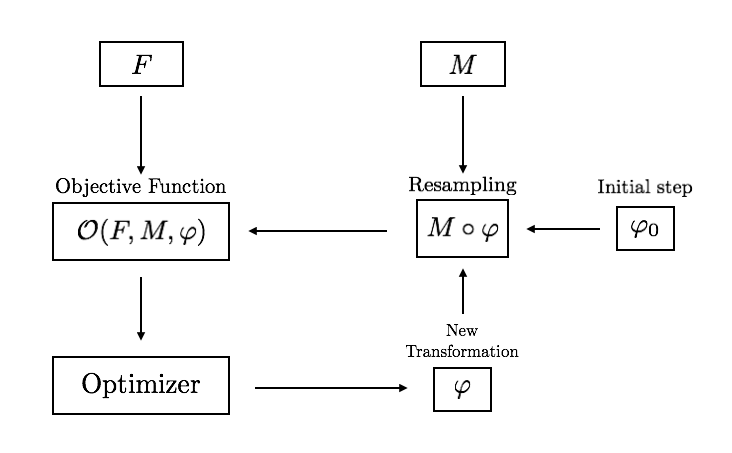
\includegraphics[scale=0.235]{figures/iterative_algorithm.png}
	\caption{Image registration framework scheme.}
	\label{fig:iterative_algorithm_scheme}
\end{figure}

\noindent
Modulating on the value of each knob, changing for example the set of transformation or the resampling technique, we change between the possible registration algorithms that generally falls in this framework.\\

\noindent
What said so far is far from being a complete overview of all of the possible frameworks; it does not take into account the fact that each version or implementation inevitably involves different needs and consequent challenges. Although it is our starting point to introduce two families of registration algorithms, the LDDMM and the demons.
For accurate surveys in medical image registration see for example \cite{Sotiras:survey:13}, \cite{zitova2003image} . \\

% % % % % % % % % % % % % % % % % % % % % % % % % % % % % % % % % % % % % %
% % SUB SECTION
% % % % % % % % % % % % % % % % % % % % % % % % % % % % % % % % % % % % % %
\subsection{LDDMM: Classic, Shooting and Stationary}\label{se:intro_lddmm}

As previously done in the elastic registration \cite{Broit:1981}, the LDDMM framework \cite{beg2005computing} originates by considering motion between images as the motion of a fluid, and utilizes ODE from fluid dynamics to compute the deformation between fixed and moving. 
% V
 A \emph{time varying vector field} (TVVF) is the continuously differentiable map defined as
 \begin{align*}
 	V:[0,1] & \longrightarrow  \mathcal{V}(\Omega)\\
 	t  &\longmapsto  V_{(t)}  : \Omega \longrightarrow   \mathbb{R}^{d} \\
 	& \qquad \quad \quad ~~~\mathbf{x} \longmapsto V_{(t,\mathbf{x} )}
 \end{align*}
 % ODE
 Once initial conditions are given, at each TVVF, corresponds a unique time varying (or non-stationary) homomorphisms defined  by the following ODE 
 \begin{align}\label{eq:ode_phi_v}
 	\frac{d\phi_{t} (\mathbf{x})}{dt} = V_{(t,\phi_{t} (\mathbf{x}) )}
 \end{align}
 % phi
 where the function $\phi$ is a path on the set of homeomorphisms  (continuous function from the background space $\Omega$ to itself with continuous inverse), indicated with $\text{Hom}(\Omega)$:
 \begin{align*}
 	\phi : [0,1] & \longrightarrow  \text{Hom}(\Omega)\\
 	t  &\longmapsto \phi_{t}  : \Omega \longrightarrow    \Omega \\
 	& \qquad \quad \quad  \mathbf{x} \longmapsto \phi_{t}  (\mathbf{x} )
 \end{align*}
%varphi
The sought transformation $\varphi$ between fixed and moving images (such that it satisfies $ F\circ \varphi^{-1} \simeq M $), is modeled in the LDDMM as the solution of the equation \ref{eq:ode_phi_v} at time $1$. Using the fundamental theorem of calculus we obtain:
 \begin{align*}
 	\varphi := \phi_{1} = \phi_{0} + \int_0^1 V_{(t,\phi_{t} (\mathbf{x}) )} dt
 \end{align*}
 % Orbits
The set of homeomorphisms is taken into account since it can define a partition of the set of images into equivalence classes, as orbits of the action on the set of images from the background space $\mathcal{I}_{\Omega}$ (see for example \cite{artin2011algebra}). In other words, given a subgroup of homeomorphisms $\mathbb{G}\subseteq \text{Hom}(\Omega)$ and an image $F$, the orbit of the action of $\mathbb{G}$ over $F$, given by
\begin{align*}
\mathcal{O}_{\mathbb{G}}(F) = \{ F\circ \varphi^{-1} \mid \varphi \in \mathbb{G} \}
\end{align*}
consists in the set of the images having the same topology of $F$.\\

%Diff, geodesics
The model proposed in the LDDMM framework imposes a first constraint in considering $\mathbb{G}$ as the set of diffeomorphisms, and a second constraint considering $\phi_{t}$ as the shortest path between the identity function on $\mathbb{G}$ and $\varphi$. In this way the resulting vector field $V_{(t,\phi_{t} (\mathbf{x}))}$ is the one that minimize the distance $l$ between transformations:
\begin{align*}
\hat{l} = \inf_{V_{(t,\phi_{t} (\mathbf{x}))} ~ : ~ \dot{\phi_{t}} (\mathbf{x}) = V_{(t,\phi_{t} (\mathbf{x}))}  
				       }
	\int_{0}^{1} \euclideanMetric{V_{(t,\phi_{t} (\mathbf{x}))}}_{L^2}^{2}dt
\end{align*}
% Sim Reg - optimization function:
For the similarity term the LDDMM uses the $L^{2}$ norm (see for example \cite{stein2009real}, chapter 4) between the moving image and the fixed image in the same orbit:
\begin{align*}
\text{Sim}(F,M,\varphi) = \frac{1}{\sigma^2}\euclideanMetric{F(\varphi^{-1})  - M  }_{L^{2}}^{2}
\end{align*}
while the regularization term is defined on the norm of the velocity vector field tangent to the transformation. Therefore, the optimization function is: 
\begin{align*}
\mathcal{E}(F, M, \varphi) 
= 
\frac{1}{\sigma^2}\euclideanMetric{F(\varphi^{-1})  - M  }_{L^{2}}^{2}
 +
\int_0^1 \euclideanMetric{L V_{(t,\phi_{t} (\mathbf{x}))} }_{L^{2}}^{2} dt
\end{align*}

% discretization 
As in many other implementation, also in the LDDMM the data structure utilized to store deformation fields are 5-dimensional matrices
\begin{align}\label{eq:basic_data_structure}
M = M(x_i,y_j,z_k,t,d) \qquad (i,j,k)\in L , ~~ t \in T  ~~ d = 1,2,3
\end{align}
where $(x_i,y_j,z_k)$ are discrete position of a lattice $L$ in the domain of the images, $t$ is the time parameter in a discretized domain $T$ and $d$ is index of the coordinate axis. So, the discretized \emph{tangent vector} $\mathbf{v}_{\tau}(x_i,y_j,z_k)$ at time $t$, has coordinates defined by
\begin{align*}
\mathbf{v}_{t}(x_i,y_j,z_k) = (M(x_i,y_j,z_k,t ,1), M(x_i,y_j,z_k,t,2), M(x_i,y_j,z_k,t ,3))
\end{align*}
% update 
At the $k$-th step, the algorithm provides the 5-dim matrix $\mathbf{v}_{k}$ that is the approximation of the discretized time varying velocity fields $V_{(t,\phi_{t} (\mathbf{x}))}$. The update at each step is computed as
\begin{align*}
\mathbf{v}_{k+1} = \mathbf{v}_{k} - \epsilon \vec{\nabla} (\Delta\mathcal{E})
\end{align*}
where $\Delta\mathcal{E}$ is the discretized version of the energy function and $\epsilon$ is the gradient descent step size.\\

% after LDDMM
% shooting
A direct upgrade of the classical LDDMM just introduced performs the optimization on the geodesic flows, defined by a set of Hamiltonian equation (Shooting LDDMM \cite{vialard2012diffeomorphic}). \\
In this algorithm the iterative evolution of the deformation field, solution of the optimization algorithm, is regularized with the constraint imposed by an additional scalar field called \emph{initial momentum}. 
%stationary: dartel and hernandez
As proved by the authors, the evaluation of this constraint at each step provides geodesics flows of homeomorphisms, but it is computationally expensive. Taking advantages of the log-Euclidean framework presented in \cite{Arsigny:MRM:06}, a subsequent algorithm called DARTEL (Diffeomorphic Anatomical Registration using Exponentiated Lie Algebra \cite{Ashburner:07}) uses a constraint based on the stationarity of the involved velocity field. Instead of considering time varying velocity fields constrained by a set of Hamiltonian equations, the domain of vector field is reduced to the stationary velocity fields, whose consequence is a considerable reduction in the computational complexity. A similar algorithm, published in contemporary with DARTEL is \cite{hernandez2007registration}, based as well on the parametrization of geodesics path of diffeomorphisms with stationary velocity fields. \\
As happened in the case of the LDDMM, the log-Euclidean framework and the use of SVF and influenced also a second family of registration algorithm, called the \emph{demons algorithm}. In 2007, a new version of the demons, based on diffeomorphisms was proposed in \cite{vercauteren2006robust}. Aim of the next section is to introduce the diffeomorphic demons algorithm, second family of algorithm that exploit diffeomorphisms for the computation of the anatomical deformations.


% % % % % % % % % % % % % % % % % % % % % % % % % % % % % % % % % % % % % %
% % SUB SECTION
% % % % % % % % % % % % % % % % % % % % % % % % % % % % % % % % % % % % % %
\subsection{Demonology: Classic, Additive, Diffeomorphic, Log and Symmetric}

% classic demonclass
The first demons-based algorithm in image registration was proposed by \cite{thirion1998image}, in analogy with the Maxwell's demon in thermodynamics. This early version - often called \emph{classic demons} - do not involves diffeomorphisms. 
The moving image is deformed with a vector field resulting from the computation of the optical flow (\cite{horn1981determining}) regularized by a gaussian filter at each step. The optical flow is based on the idea that a voxel in the moving image is attracted by some force to all the points in the fixed with similar intensity. \\

The final deformation, solution of the registration problem is obtained composing at each step the previous transformation with an update: let $\{T_{k}\}_{k=1}^{N}$ be the sequence of deformation and let $\delta T_{k}$ be the update at the step $k$. They can be expressed as the identity plus the displacement field $V$:
\begin{align*}
	T_{k}(\mathbf{x}) &= \mathbf{x} + V_{k}(\mathbf{x}) \\ 
	\delta T_{k}(\mathbf{x}) &= \mathbf{x} + \delta V_{k}(\mathbf{x}) 
\end{align*}
And the $k$-th deformation is computed by composition as:
\begin{align*}
T_{k+1}(\mathbf{x})  :&= (\delta T_{k}\circ T_{k})(\mathbf{x}) \\
&= \mathbf{x} + \delta V_{k}(\mathbf{x}) + V_{k}(\mathbf{x} + \delta V_{k}(\mathbf{x}))
\end{align*}
Since the third addend is close to $V_{k}(\mathbf{x})$, some implementation - as for example ITK - consider only the sum between 
$ V_{k+1}$ and $V_{k}$ in the computation of the update:
\begin{align*}
T_{k+1}(\mathbf{x})  :&= (\delta T_{k} + T_{k})(\mathbf{x}) \\
&= \mathbf{x} + V_{k}(\mathbf{x}) + \delta V_{k}(\mathbf{x})
\end{align*}
Demons algorithms with this implementation are often called \emph{additive demons}.\\

%PASHA
In the paper that presents the PASHA demons \cite{cachier2003iconic}, authors point out the fact that the classic demon is based on the minimization of a local energy function that sees each voxel independent from each others. In consequence of this limitation the authors of the PASHA reformulate the algorithm using a global energy function, aimed to make the method based on a global energy function, and therefore easier to be analyzed and compared with other methods. With some modifications, the Classic demons algorithm is accompanied back to the framework presented in the previous section, having a global energy function which optimization provides at each step the update of the transformation. \\

It is important to notice that the PASHA algorithm does not involve any diffeomorphism. The solution is smoothed with the widespread stratagem of applying a Gaussian filter $G$ at each of the global transformation $T_{k}$ involved in the registration:
\begin{align*}
T_{k+1}(\mathbf{x})  &:= G_{1}(T_{k}(\mathbf{x}) + G_{2}(\delta T_{k}(\mathbf{x}))
\end{align*}
% smoother as gaussian
In general if $G_{1}$ is omitted the model is sometime called \emph{fluid}, while if $G_{2}$ is omitted is called \emph{elastic}.\\

Diffeomorphisms were introduced within the demons algorithm (\emph{diffeomorphic demons} \cite{vercauteren2006robust}) after the presentation of the log-Euclidean framework \cite{Arsigny:MRM:06}. 
To each stationary velocity field $V \in \mathcal{V}(\Omega)$ is associated a diffeomorphisms $\varphi$ by the ODE $d\varphi /dt = V_{(t,p)} $.\\
Using Lie theory, SVF are elements of the \emph{Lie algebra} - usually denoted with $\mathfrak{g}$ - while the set of diffeomorphisms are elements of the Lie group - denoted with $\mathbb{G}$ -.\\

Roughly speaking, the Lie algebra $\mathfrak{g}$ is the tangent space (as local linear approximation) to the Lie group $\mathbb{G}$, and these two spaces are in local correspondence thanks to two \lq\lq crossing-structure\rq\rq~ functions: the \emph{Lie exponential} and the \emph{Lie logarithm}. \emph{Lie exponential} maps vector fields on the corresponding Lie group elements, while the \emph{Lie logarithm} - inverse of the Lie exponential under some condition, see \cite{do1976differential} or \cite{lee2012introduction} - maps each diffeomorphisms in the correspondent tangent vector field:
\begin{align*}
\varphi = \exp(V)  
\quad
V = \log(\varphi ) 
\qquad \qquad
\varphi  \in \mathbb{G}
\quad
V \in \mathfrak{g}
\end{align*}
In this settings, the update can not be computed simply with a sum of vector fields, since it must reflect the composition of the corresponding diffeomorphisms in the Lie group.\\


Several approaches has been presented to face the problem of the computation of the update. Diffeomorphic demons compute the transformation at each step of the iterative algorithm as the composition between the diffeomorphism $\varphi_{k}$ obtained at the previous step with the exponential of the SVF $\delta V_{k}$, obtained with the optimization algorithm:
\begin{align*}
\varphi_{k + 1} := \varphi_{k}  \circ \exp(\delta V_{k})
\end{align*}
In a subsequent version, the log-demons \cite{vercauteren08}, the composition is performed in the tangent space toward exponential and logarithm functions
\begin{align}\label{eq:bch_problem}
V_{k + 1} := \log( \exp(V_{k})  \circ \exp(\delta V_{k}))
\end{align}
For this last computation, another treasure from the theory of Lie group has been stolen: the BCH formula. It provides the solution for $Z$ of the equation 
\begin{align*}
 \exp(Z) = \exp(X)\circ\exp(Y)
\end{align*}
Its solution involves an infinite series of nested Lie bracket, that do not makes its computation straightforward. 
To face the problem of its numerical approximation, whose solutions are utilized to solve \ref{eq:bch_problem}, we define in this thesis a binary operation called log-composition.


% % % % % % % % % % % % % % % % % % % % % % % % % % % % % % % % % % % % % %
% % SECTION
% % % % % % % % % % % % % % % % % % % % % % % % % % % % % % % % % % % % % %
\section{The Log-composition at the Service of Image Registration}

Every non-rigid registration algorithm requires to be implemented and to work with discretized images.
The nature of the computers' memory prevent from the possibility of storing the continuous fluid transformations that, for example, solves the differential equations of the LDDMM or any of the diffeomorphisms resulting from the demons. The only manipulations we are allowed to perform, are storing the discretized vector fields and resampling them using one of the available techniques.\\
% why log composition:
When relying on diffeomorphic algorithms, we still have to consider discretized vector fields as elements of a Lie algebra whose Lie group appears to be a support for the computation of their composition in the equation \ref{eq:bch_problem}.
This operation of composition of tangent vector fields, based on the diffeomorphisms is baptized here under the name of \emph{log-composition} and it is defined as
\begin{align*}
X \oplus Y := \log(\exp(X)\circ\exp( Y))
\qquad \qquad
\forall ~X, Y \in \mathfrak{g}
\end{align*}
The main aim of this document is to present a comparison between numerical methods for its computation. \\

% where we can use the log composition
It is worthed to notice that a fast and accurate computation of the log-composition may not influence only the diffeomorphic demons. It may be used as well in medical imaging for
\begin{enumerate}
	\item Symmetric diffeomorphic demon \cite{vercauteren08}.
	\item Fast computation of the logarithm \cite{Bossa:08} (discussed in chapter \ref{ch:log_algorithm}).
	\item Calculus on diffusion tensor \cite{Arsigny:MRM:06}. 
	\item Compute the discrete ladder for Parallel Transport in Transformation Groups \cite{Lorenzi:discrete_ladders:14}.
\end{enumerate}	
	
The next chapter is aimed to the formal definition of the log-composition, underpinned with the tools from differential geometry theory and to present two new numerical technique to compute it.


